\documentclass[10pt]{article}

\usepackage{mathtools}  % need for math tools
\usepackage{amsmath}    % need for subequations
\usepackage{graphicx}   % need for figures
\usepackage{verbatim}   % useful for program listings
\usepackage{color}      % use if color is used in text
\usepackage{subfigure}  % use for side-by-side figures
\usepackage{hyperref}   % use for hypertext links, including those to external documents and URLs
\usepackage{graphicx}   % Used to import the graphics

\setlength{\baselineskip}{16.0pt}   
\setlength{\parskip}{3pt plus 2pt}
\setlength{\parindent}{20pt}
\setlength{\oddsidemargin}{0.5cm}
\setlength{\evensidemargin}{0.5cm}
\setlength{\marginparsep}{0.75cm}
\setlength{\marginparwidth}{2.5cm}
\setlength{\marginparpush}{1.0cm}
\setlength{\textwidth}{150mm}



\begin{document}

\begin{center}
{\large Ay190: Computational Astrophysics (Winter Term 2012)} \\
{\large HomeWork - 2 } \\
\copyright 2012 by Arya Farahi \\
Jan 10, 2012
\end{center}

\section{Exercise 1. Finite Difference Approximation and Convergence}

\begin{figure}[hbt]
  \begin{center}
    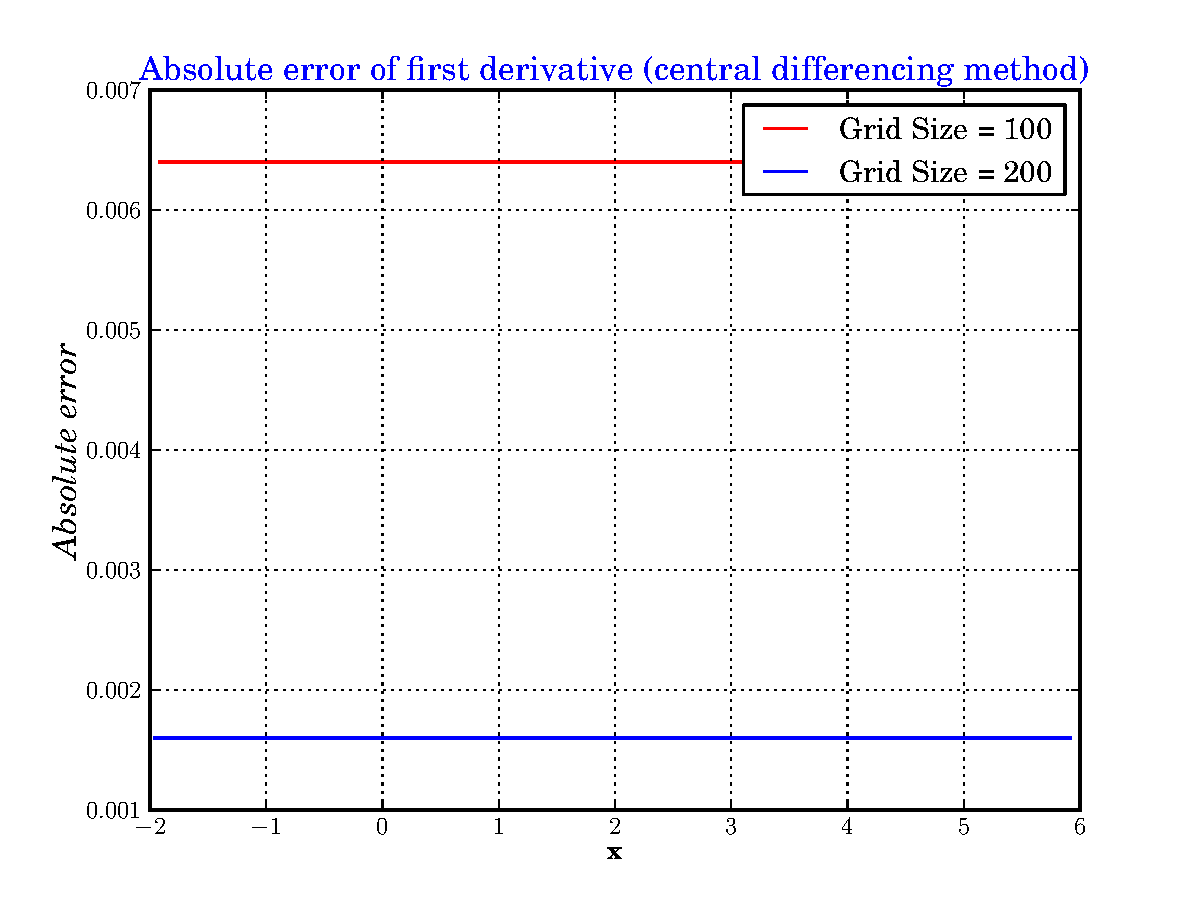
\includegraphics[scale=0.5]{Plots/plot1.pdf}
    \caption{\label{fig:ForwardMethod} Plot of the absolute error of first derivative with forward method for 200 and 100 cell grid size.}
  \end{center}
\end{figure}


\begin{figure}[hbt]
  \begin{center}
    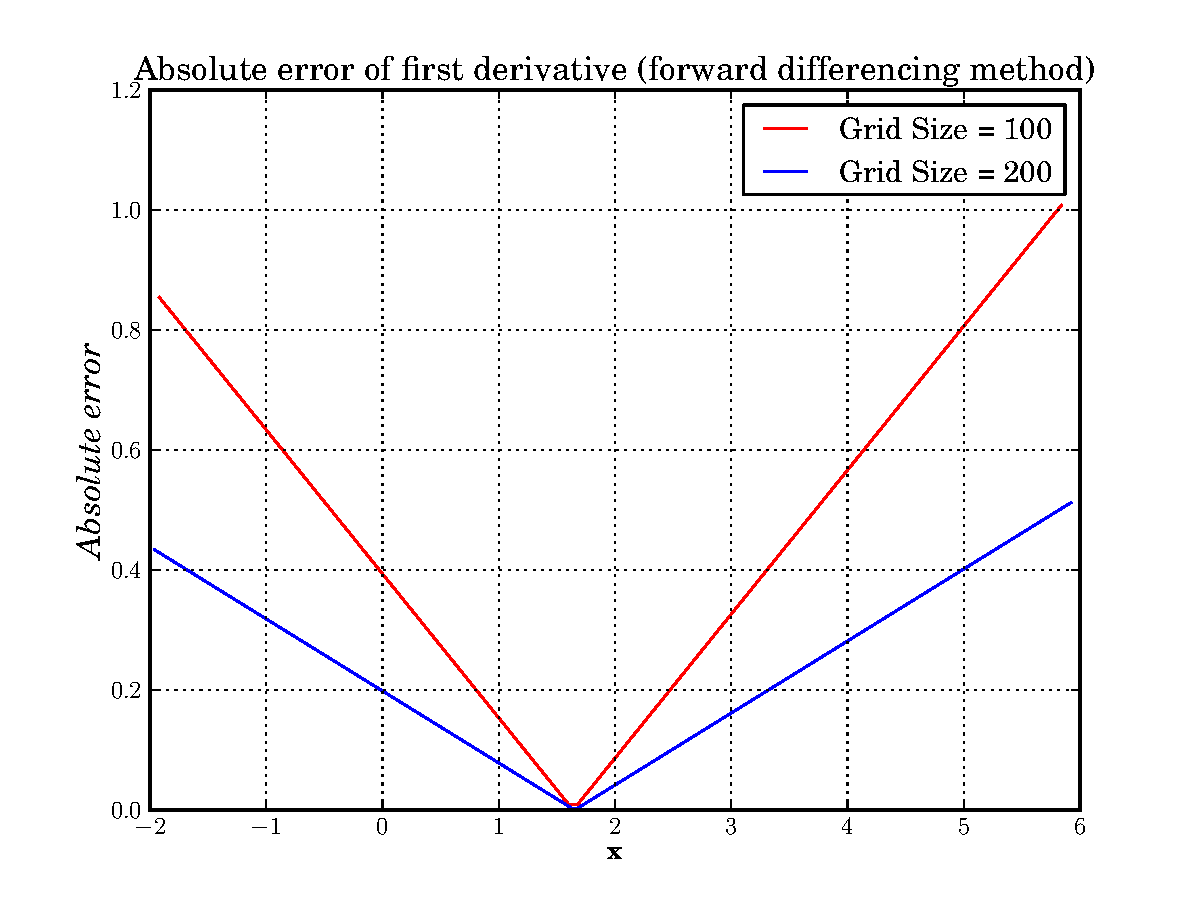
\includegraphics[scale=0.5]{Plots/plot2.pdf}
    \caption{\label{fig:CentralMethod} Plot of the absolute error of first derivative with forward method  with central method for 200 and 100 cell grid size.}
  \end{center}
\end{figure}

\begin{figure}[hbt]
  \begin{center}
    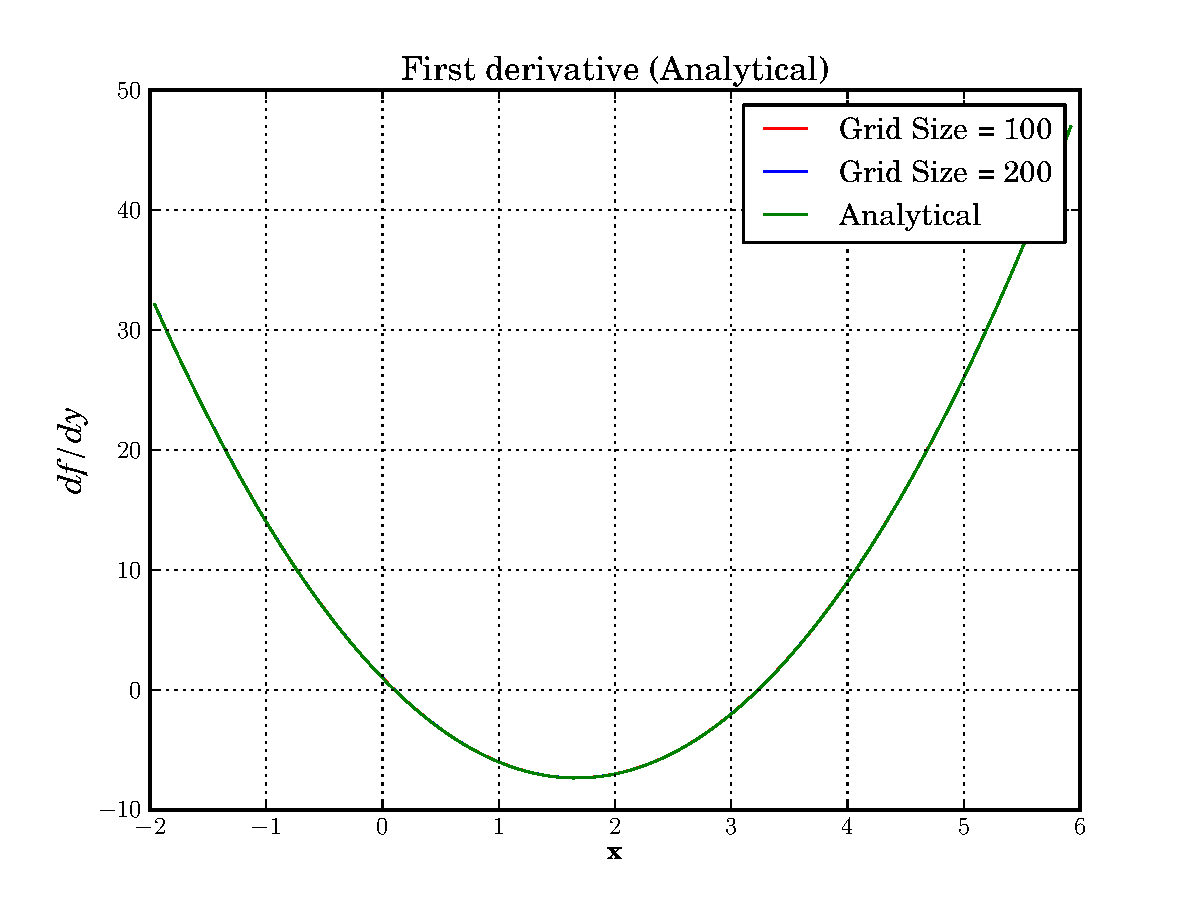
\includegraphics[scale=0.5]{Plots/plot3.pdf}
    \caption{\label{fig:ForwardMethoddf/dx} Plot of first derivative with forward method for 200 and 100 cell grid size.}
  \end{center}
\end{figure}


\begin{figure}[hbt]
  \begin{center}
    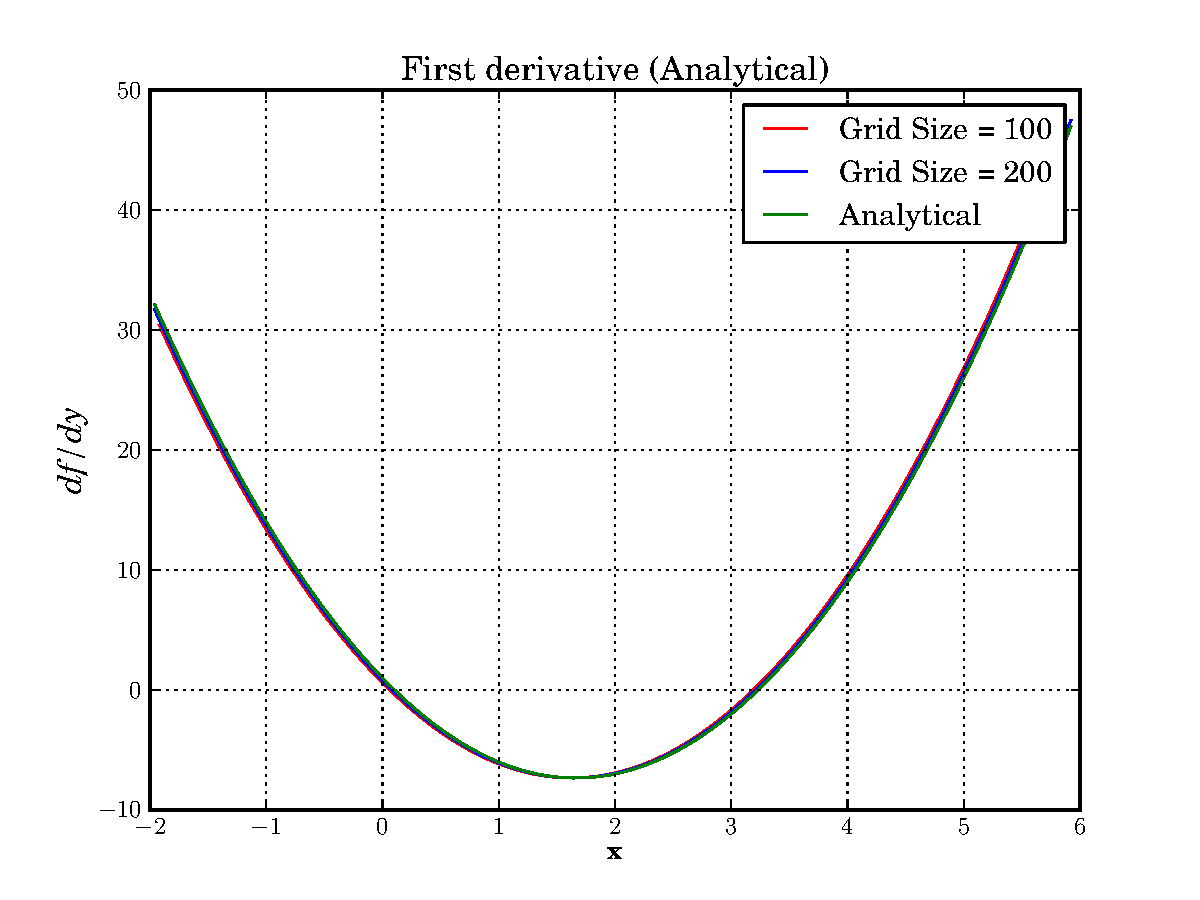
\includegraphics[scale=0.5]{Plots/plot4.pdf}
    \caption{\label{fig:CentralMethoddf/dx} Plot of first derivative with forward method with central method for 200 and 100 cell grid size.}
  \end{center}
\end{figure}

figure \ref{fig:ForwardMethod} showes the plot of absolute error of first derivative with forward method for two different grid size. (100 and 200 cell grid size) and figure \ref{fig:CentralMethod} showes the plot of absolute error of first derivative with central method for two different grid size. (100 and 200 cell grid size) \\


figure \ref{fig:ForwardMethoddf/dx} showes the plot of first derivative with forward method for two different grid size. (100 and 200 cell grid size) and figure \ref{fig:CentralMethoddf/dx} showes the plot of first derivative
with central method for two different grid size. (100 and 200 cell grid size) \\


As it is shown in the figure \ref{fig:ForwardMethod} and \ref{fig:CentralMethod} the absolute error for forward method get decreased with relation $\frac{(ABS-ERR)_1}{(ABS-ERR)_2} = \frac{1}{2}$ and for central method $\frac{(ABS-ERR)_1}{(ABS-ERR)_2} = \frac{1}{4}$  as we expected. So we can conclude that these methods converges to first derivative of our function.\\


\section{Exercise 2. Finite Difference Approximation and Convergence}

By teylor expansion we can derive the following equations:\\

\begin{equation}\label{eq:eq11}
 f(x_0+h) = f(x_0) + hf'(x_0) + h^2f''(x_0)/2 + h^3f'''(x_0)/6 + \mathcal{O}(h^4_o)  
\end{equation}

and\\

\begin{equation}\label{eq:eq22}
 f(x_0-h) = f(x_0) - hf'(x_0) + h^2f''(x_0)/2 - h^3f'''(x_0)/6 + \mathcal{O}(h^4_o)  
\end{equation}

Simply by adding the equation number \ref{eq:eq11} and \ref{eq:eq22} we can derive the following formula:\\

\begin{equation}
f''(x_0) = \frac{f(x_0+h) - 2f(x_0) + f(x_0-h)}{ h^2}  + \mathcal{O}(h^2_o)  
\end{equation}


\section{Exercise 3. Interpolation: Cepheid Lightcurve}


Figure \ref{fig:Interpol} shows the interpolation of Cepheid Lightcurve with piecewise linear, piecewise quadratic, Lagrange, Cubic Hermit, and Cubic Spline methods. It is obviuse that for this set of datas Lagrange and Cubic Hermit methods are not a good appraximation for intepolating the Cepheid Lighcurve function so we need to use the other methods for finding the interpolation. Figure \ref{fig:Interpol2} shows just answer of interpolation Cepheid Lightcurve with piecewise linear, piecewise quadratic, Cubic Spline methods. With this set of data quadratic interpolation is the best method for finding the missing values. \\

\begin{figure}[hbt]
  \begin{center}
    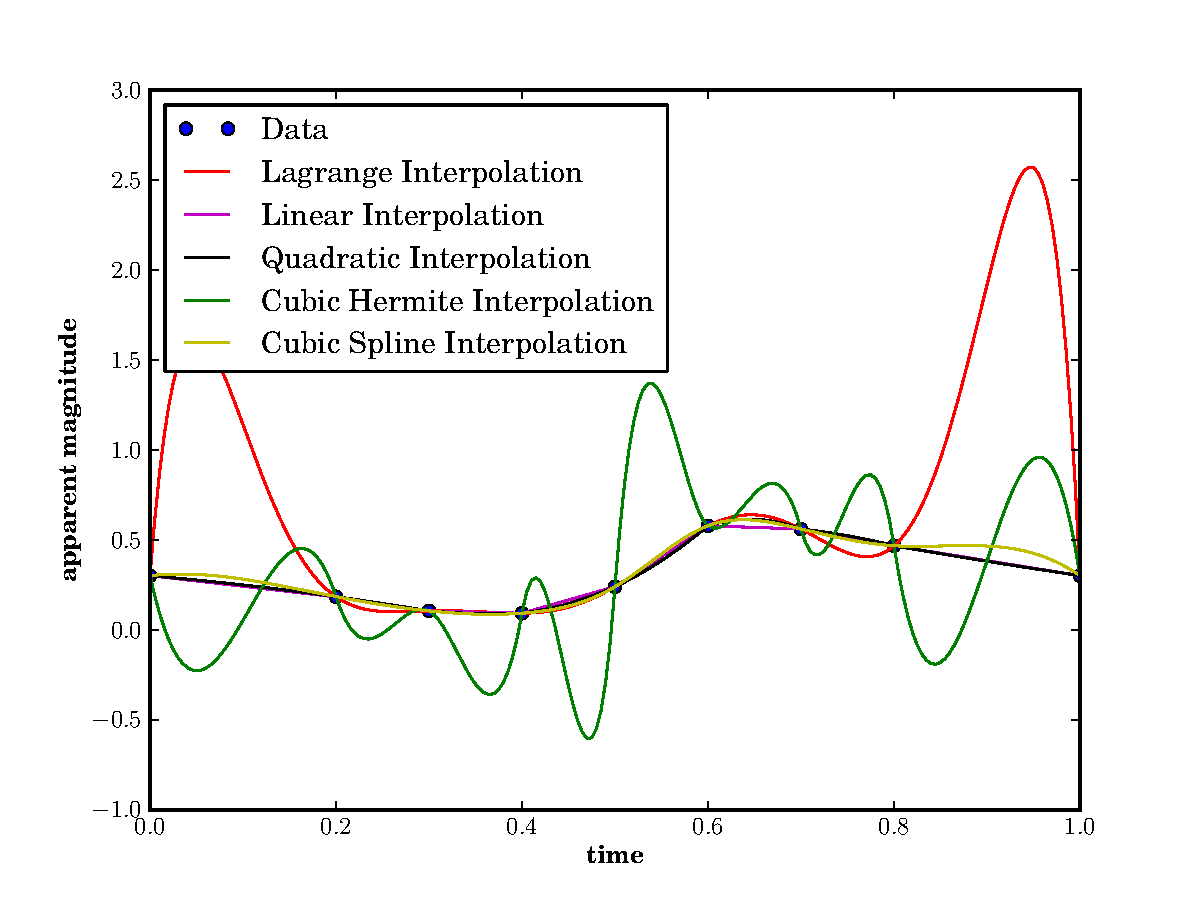
\includegraphics[scale = 0.5]{Plots/plot5.pdf}
    \caption{\label{fig:Interpol} Interpolation of Cepheid Lightcurve with different methods.}
  \end{center}
\end{figure}
  

\begin{figure}[hbt]
  \begin{center}
    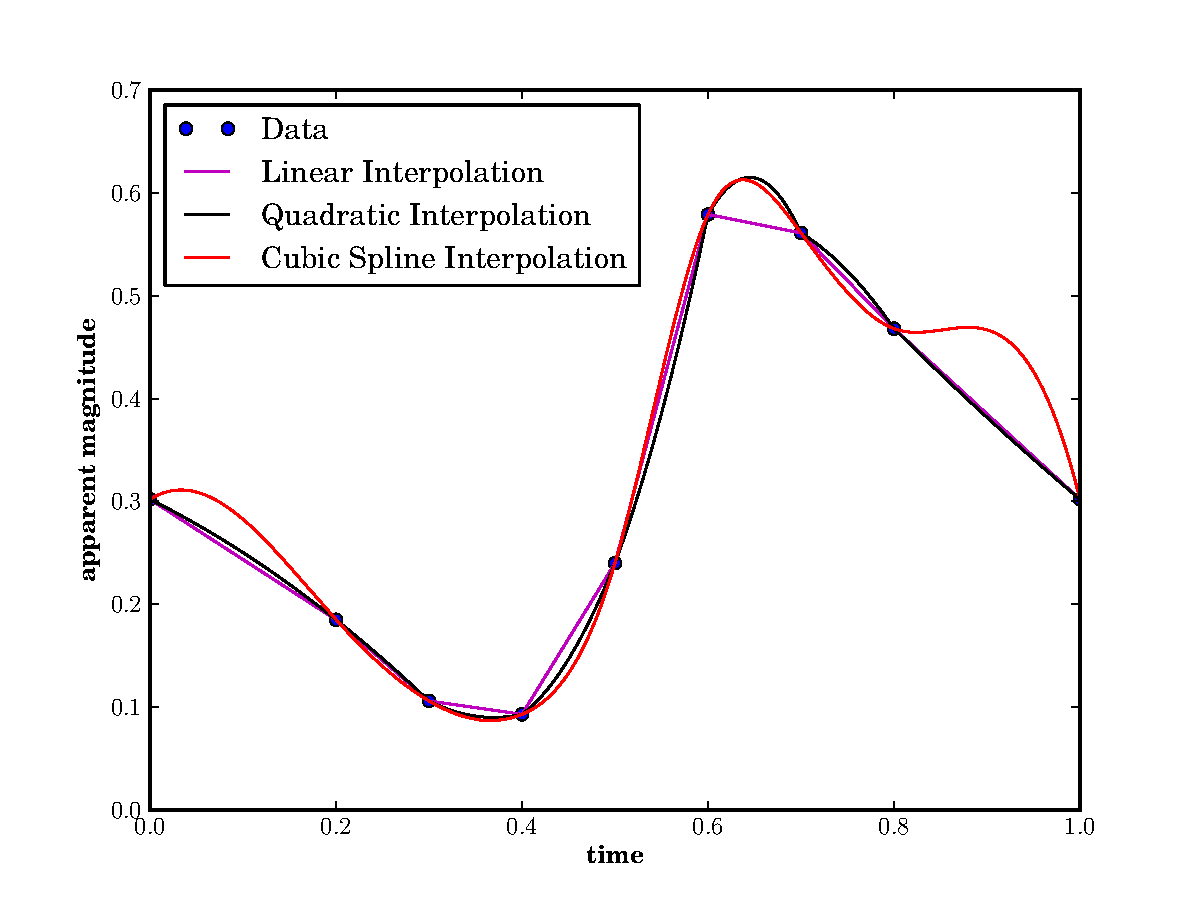
\includegraphics[scale = 0.5]{Plots/plot6.pdf}
    \caption{\label{fig:Interpol2} Interpolation for Cepheid Lightcurve with piecewise linear, piecewise quadratic, and cubic spline methods.}
  \end{center}
\end{figure}


\end{document}
